%%%--- Template for master thesis at SfS
%%%--- Modified template with more comments and examples -- SG, 11/06/09
%%%------
\documentclass[11pt,a4paper,twoside,openright]{report}
\usepackage[english]{ETHDAsfs}%--> ETHDASA + fancyhdr + ... "umlaute"
%  + sfs-hyper -> hyperref 

\usepackage{pdfpages}%%to include the confirmation of originality (plagiarism
\usepackage{amsbsy}%% for \boldsymbol and \pmb{.}
\usepackage{amssymb}%% calls  amsfonts...
\usepackage{graphicx}%-- für PostScript-Grafiken (besser als  psfig!)
%\usepackage[draft]{graphicx} % grafics shown as boxes --> faster compilation
%
\usepackage[longnamesfirst]{natbib}%was {sfsbib}%- Für  Literatur-Referenzen
%           ^^^^^^^^^^^^^^ 1) "Hampel, Ronchetti, ..,"  2) "Hampel et al"
% Engineers (and other funny people) want to see [1], [2] 
% ---> use 'numbers' : \usepackage[longnamesfirst,number]{natbib}
%
%
\usepackage{texab}%- 'tex Abkürzungen' /u/sfs/tex/tex/latex/texab.sty
        %%- z.B.  \R, \Z, \Q, \Nat für reelle, ganze, rationale, natürl. Zahlen;
        %%-       \N   (Normalvert.)  \W == Wahrscheinlichkeit .....
        %%-  \med, \var, \Cov, \....
        %%-  \abs{x} == |x|   und   \norm{y} ==  || y ||   (aber anständig)
%% NOTE: texab contains many useful definitions and "shortcuts". It is
%% worth to open the file and have a look at them. HOWEVER, some
%% definitions are a bit can lead to conflicts with other packages. You
%% might for example want to comment out the line defininf \IF as an
%% operator when working with the algorithmic package, or to comment out
%% the line defining a command \Cite with working with the Biblatex package  
\usepackage{amsmath}
%\usepackage{mathrsfs}% Raph Smith's Formal Script font --> provides \mathscr
\usepackage[utf8]{inputenc}% <<------- Unicode, *NOT* iso-latin1 !
\usepackage{ae}% A[lmost] E[uropean] Fonts
\usepackage{enumerate}% Fuer selbstdefinierte Nummerierungen
%--------
\usepackage{relsize}%-> \smaller (etc) used here
\usepackage{color} %% to allow coloring in code listings
\usepackage{listings}% Fuer R-code, C-code, ....  and settings for these:
\definecolor{Mygrey}{gray}{0.75}% for linenumbers only!
\definecolor{Cgrey}{gray}{0.4}% for comments
\lstloadlanguages{R}
%%--- first version of "listings of R"-style : ---------------------------
% %% using \smaller here: makes R code listings use a *small* font:
% \lstset{language=R,basicstyle=\smaller[2],commentstyle=\rmfamily\smaller,
%   showstringspaces=false,xleftmargin=4ex,
%   literate={<-}{{$\leftarrow$}}1 {~}{{$\sim$}}1}
% \lstset{escapeinside={(*}{*)}} % for (*\ref{ }*) inside lstlistings (Scode) 
%\newcommand{\lil}[1]{\lstinline|#1|}
%%--- newer version of "listings of R"-style : ---------------------------
\lstset{%% Help, e.g. --> https://en.wikibooks.org/wiki/LaTeX/Source_Code_Listings
language=R,
basicstyle=\ttfamily\scriptsize,%%- \small > \footnotesize > \scriptsize > \tiny
%commentstyle=\ttfamily\color{Cgrey},
commentstyle=\itshape\color{Cgrey},
numbers=left,
numberstyle=\ttfamily\color{Mygrey}\tiny,
stepnumber=1,
numbersep=5pt,
backgroundcolor=\color{white},
showspaces=false,
showstringspaces=false,
showtabs=false,
frame=single,
tabsize=2,
captionpos=b,
breaklines=true,
%breakatwhitespace=false,
keywordstyle={},
morekeywords={},
xleftmargin=4ex, 
literate={<-}{{$\leftarrow$}}1 {~}{{$\sim$}}1}
\lstset{escapeinside={(*}{*)}} % for (*\ref{ }*) inside lstlistings (Scode) 
%%----------------------------------------------------------------------------

%%------- Theoreme ---
\newtheorem{definition}{Definition}[subsection]
\newtheorem{lemma}[definition]{Lemma}
\newtheorem{theorem}[definition]{Theorem}
\newtheorem{Coro}[definition]{Corollary}
\theoremstyle{definition} 
\newtheorem{example}[definition]{Example}
\newtheorem*{note}{Note}
\newtheorem*{remark}{Remark}

\DeclareMathOperator*{\plim}{plim}
% \def\MR#1{\href{http://www.ams.org/mathscinet-getitem?mr=#1}{MR#1}}

% \newcommand{\Lecture}[3]{\marginpar{#3.#2.#1}}
% \newcommand{\Fu}{\mathcal{F}}
\newcommand{\aatop}[2]{\genfrac{}{}{0pt}{}{#1}{#2}}

%\renewcommand{\theequation}{\arabic{equation}}
\numberwithin{equation}{subsection}

%%%%%%%%%%%%%%%%%%%%%%%%%%%%%%%%%%%%%%%%%%%%%%%%%
%%% Path for your figures                      %%%
%%%%%%%%%%%%%%%%%%%%%%%%%%%%%%%%%%%%%%%%%%%%%%%%%
% Set the paths where all figures are taken from:
\graphicspath{{Pictures/}}

%%%%%%%%%%%%%%%%%%%%%%%%%%%%%%%%%%%%%%%%%%%%%%%%%
%%% Define your own commands here             %%%
%%%%%%%%%%%%%%%%%%%%%%%%%%%%%%%%%%%%%%%%%%%%%%%%%
\newcommand{\Bruch}[2]{{}^{#1}\!\!/\!_{#2}}
\renewcommand{\labelenumi}{\roman{enumi}.)}



\begin{document}
\bibliographystyle{chicago}% ---> Hampel,F., E.Ronchetti,... W.Stahel(1986) ...
 %was \bibliographystyle{sfsbib}\citationstyle{dcu} %OR DEFAULT : \citationstyle{agsm}

\pagenumbering{roman}%- roman numbering for first few pages

%%%%%%%%%%%%%%%%%%%%%%%%%%%%%%%%%%%%%%%%%%%%%%%%%
%%% Title page                                %%%
%%%%%%%%%%%%%%%%%%%%%%%%%%%%%%%%%%%%%%%%%%%%%%%%%
\period{Summer 2023}
\dasatype{Master Thesis}
\students{Student Muster}
\mainreaderprefix{Advisor:}
\mainreader{Prof.\ Dr.\ Your supervisor}
\alternatereaderprefix{Co-Advisor}
\alternatereader{Your co-supervisor}
\submissiondate{13 March 2023}
\title{Time Series Analysis \\ for Irregularly Sampled Data }

\maketitle%- Titelseite wird abgeschlossen
\cleardoublepage
 %%~~~~~~~~~~~~~~~~~~~~~~~~~~~~~~~~~~~~~~~~

%%%%%%%%%%%%%%%%%%%%%%%%%%%%%%%%%%%%%%%%%%%%%%%%%
%%% Insert here acknowledgements and abstract %%%
%%%%%%%%%%%%%%%%%%%%%%%%%%%%%%%%%%%%%%%%%%%%%%%%%
%% Dedication (optional)
\markright{}
\vspace*{\stretch{1}}
\begin{center}
    To some special person
\end{center}
\vspace*{\stretch{2}}

% Preface (optional)
\newpage
\markboth{Preface}{Preface}
\chapter*{Preface}

% TODO uncomment
%Thank you Dr. Markus Kalisch for your exceptional
%supervision, for being very open to my ideas but also providing invaluable
%guidance and generally for the enthusiasm to discover the realm of Gaussian
%processes.
%
%Thank you, Dr. David Perruchoud for your consistent support throughout the
%thesis, for helping me to come up with the research topic and
%to always ask the questions that would keep me on track.
%
%My appreciation also goes to Dr. Josep Sola and the entire Aktiia team for
%their attentive ears, valuable feedback on my research findings and for
%the office space right next to Limmat.
%
%



% Abstract should not be longer than one page.
\newpage
\markboth{Abstract}{Abstract}
\chapter*{Abstract}

Short summary of my thesis.
 

%%% Local Variables: 
%%% mode: latex
%%% TeX-master: "MasterThesisSfS"
%%% End: 


%%%%%%%%%%%%%%%%%%%%%%%%%%%%%%%%%%%%%%%%%%%%%%%%%
%%% Table of contents and list of figures and %%%   
%%% tables (no need to change this usually)   %%%
%%%%%%%%%%%%%%%%%%%%%%%%%%%%%%%%%%%%%%%%%%%%%%%%%
\newpage
\tableofcontents
\newpage
\listoffigures
\newpage
\listoftables

%% Notations and glossary (optional)
\cleardoublepage
\phantomsection
\addcontentsline{toc}{chapter}{\protect\numberline{}{Notation}}
\markboth{Notation}{Notation}
\chapter*{Notation}
\label{c:Notation}


\section{General Statements}
Prediction: Estimation of the expected time series value at some time
$x^{\ast}$, with $x^{\ast}$ being within the time range of available observations.
\\
Forcasting: Estimation of the expected time series value at some time
$x^{\ast}$, with $x^{\ast}$ being after the last available observations \\
Vectors are column vectors unless stated otherwise.

\section{Abbreviation}\label{sec:abbreviation}
GP: Gaussian process. \\
BP: Blood pressure. \\
CI: Refers to both confidence and credible interval\\
OLS: Ordinary Least Squares. \\
iid: Independent and identically distributed.

\section{Symbols}\label{sec:symbols}
$\mathcal{N}(\mu,\,\sigma^{2})$ : Normal distribution with mean $\mu$ and standard deviation $\sigma$ \\
$X_1 \dots X_n \iidsim F$ : $X_1 \dots X_n$ are iid with distribution $F$ \\
$|M|$: determinant of matrix $M$ \\
$\ERW{X}$: Expectation of X \\
$\COV{X,Y}$: Covariance between $X$ and $Y$ \\
$\VAR{X}$: Variance of X


%%% Local Variables: 
%%% mode: latex
%%% TeX-master: "MasterThesisSfS"
%%% End: 

\cleardoublepage
\pagenumbering{arabic}%--- switch back to standard numbering 


%%%%%%%%%%%%%%%%%%%%%%%%%%%%%%%%%%%%%%%%%%%%%%%%%
%%% Your text... Either write here directly,  %%%
%%% or even better: write in separate files   %%%
%%% that you just have to include here.       %%% 
%%%%%%%%%%%%%%%%%%%%%%%%%%%%%%%%%%%%%%%%%%%%%%%%%
%! Author = gianna
%! Date = 05.04.23
\chapter{Introduction}\label{ch:introduction}


\section{Thesis Objective}\label{sec:thesis-objective}

The thesis aims at giving an overview of time series analysis methods for irregularly sampled data.

The standard time series analysis methods usually assume discrete equispaced time and introductory textbooks on
time series analysis either completely omit the irregularly spaced case or they only dedicate
a very small section to continuous time models or to state-space models
with missing observations (\citeauthor{brockwell_time_1991}, \citeauthor{brockwell_introduction_2016},
\citeauthor{cryer_time_2008}, \citeauthor{chatfield_analysis_2003}).

I will thereafter present the most important concepts and what I have identified to be the basic methods for
the analysis of irregularly spaced time series.

The topic is motivated by a "real world" problem from medicine.
%
%Motivated by a "real world" problem from medicine, I have tried to identify the most important concepts and basic
%methods for the analysis of irregularly space time series, which I will be presented in this thesis.
The problem at hand is the one of extracting time series characteristics from a dataset
featuring blood pressure (BP) measurements sampled at irregularly spaced time points.
High BP is known to be a risk factor for cardiovascular disease.
A person’s BP level is generally summarized using the average BP value over available measurements within a given time range.
A novel monitoring device already allows to collect BP estimates round the clock.
The device is collecting photoplethysmography (PPG) signals and converting them into BP measurements.
Typically, the system will yield approximately 1.5 BP measurements per hour, but depending on the quality of the PPG signal and some additional external factors,
this sampling frequency can widely vary and the expected range lies roughly between 0 and 5 measurements per hour.
Having good estimates of the true BP values at any, potentially not observed, time would allow for a better estimation
of the person’s cardiovascular risk, and enable the development of novel valuable metrics.
The thesis will focus on a set of time series characteristics, which have been considered most relevant for estimating
the person’s cardiovascular risk.
The characteristics of interest are:
\begin{itemize}
    \item the mean function of the BP time series
    \item the one-week mean BP value
    \item any "long-term" trends
    \item characteristics of the circadian cycle, such as the mean day and night BP
\end{itemize}
Besides the point estimates also their CIs are of interest.
Importantly, the CI should be able to capture the uncertainty due to the lack of data in the proximity of the point of prediction.
This implies, that the width of the CI intervals around the mean function will not be constant over time but depend, among
other factors, on how much data is available in the proximity of a given time point.
The described endpoints are all based on prediction at the not observed passed time points however not on forcasting at new time points in
the future.
Hence, the thesis will only focus on the task of reconstructing BP values between the first and last time point in the dataset.

This "real world" problem will serve as a running example throughout the Thesis.
Although the topic is motivated by a real dataset we will restrict ourselves to simulated data,
which will mimic the most important characteristics of BP time series data.


\section{Thesis Outline}

TODO










%%% Local Variables: 
%%% mode: latex
%%% TeX-master: "MasterThesisSfS"
%%% End: 

%! Author = gianna
%! Date = 06.04.23


\chapter{Characteristics of Time Series}

A \textbf{time series} $(x_t)$ is a collection of observations $x_t$ ,
each one being recorded at a specific time $t \in T_0$.
$T_0$ is the set of times at which observations are made.
In case of discrete time series $T_0$ is a discrete set, e.g. for the equispaced case $T_0 = \{1, 2, \dots T\}$ and
for the unequally spaced case $T_0 = \{t_1, t_2, \dots t_n\}$ with $t_1 < t_2 < \dots t_n$.
For continuous time series $T_0$ is an interval, e.g. $T_0 = [1, T]$.

A \textbf{time series model} for the observed data $(x_t)$ is specified by the collection of random variables
$(X_t)$ of which $(x_t)$ is thought to be a realization.
Alternatively the time series model can also be considered a random function $f: T_0 \to \mathbb{R}$.

Throughout the thesis the term time series is used both refer to the data and the process from which it is generated.

%a specification of the joint
%distributions (or possibly only the means and covariances) of a sequence of random
%variables ${X_t}$ of which ${x_t}$ is postulated to be a realization.

\textbf{mean function}

\textbf{autocovariance function}


\section{Stationarity}
Stationarity is needed for being able to statistically learn from time series data.



\section{ARMA Model}

Autoregressive Process
Moving Average Process



\section{Characteristics of the Blood Pressure Time Series}

circadian cycle







%! Author = gianna
%! Date = 06.04.23


\chapter{Time Series Decomposition and Regression}\label{ch:time-series-decomposition-and-regression}

%Many authors use the word trend only for a slowly changing mean func-
%tion, such as a linear time trend, and use the term seasonal component for a mean func-
%tion that varies cyclically.


As most time series, the mean function of the BP time series is not constant in time and hence it is not stationary.
One can try to decompose the time series $Y(t)$ into a deterministic component, the mean function $\mu(t)$
and a zero mean stationary process $E(t)$. This can be expressed in the form of a regression problem:

\[ Y(t)= \mu(t) + E(t) \]

The decomposition allows to extract a stationary component $E(t)$, for which we can find a probabilistic model
using the theory of such stationary time series processes. The idea is to then use this model in combination
with an estimate of $\mu(t)$ to obtain a probability distribution of $Y^{\ast}$ at some time $t^{\ast}$.
Hence time series decomposition comes for free in regression analysis and we start with estimation of
the deterministic component $\mu(t)$ which might be an arbitrary function of $t$.

\section{Linear Regression}\label{sec:linear-regression}
Based on the knowledge we have about the system we might restrict ourselves to a family of function for $\mu(t)$.
An obvious choice for the BP time series is the family of functions featuring a linear trend
with an additive seasonal component.
If the seasonal component is represented by a cosine of the form $\alpha \cos(2 \pi f t - \phi)$ with phase shift $\phi$
and known frequency $f$, we get the following model for the BP time series $Y(t)$:
\begin{gather*}
Y(t) = \beta_0 + \beta_1 t + \beta_2 \cos(2 \pi f t) + \beta_3 \sin(2 \pi f t) + E(t), \\
\end{gather*}
where based on the trigonometric angle sum identities we know that $\beta_2 = \alpha \cos(\phi)$ and $\beta_3 = \alpha \sin(\phi)$.

If we assume BP observations at potentially unequally spaced
time points $t_1, t_2 \dots t_n$ and $t_1 < t_2 < \dots t_n$, we can write in matrix notation:
\begin{gather*}
\mathbf{Y} = X \beta + \mathbf{E}
\end{gather*}

Where $\mathbf{Y} = [Y_{t_1}, \dots Y_{t_n}]^{\top}$ is the observed time series,
$X = [x_{t_1}, \dots x_{t_n}]^{\top} \in \mathbb{R}^{n \times 4}$ is the design matrix with i-th row
$x_{t_i} = [1, t_i, \cos(2 \pi f t_i), \sin(2 \pi f t_i)]^{\top}$
and $\mathbf{E} = [E_{t_1}, \dots E_{t_n}]^{\top}$ the zero-mean stationary time series,
which we will call errors.

We can use ordinary least squares to find unbiased and asymptotically normal estimates $\hat{\beta}_{OLS} = (X^{\top}X) X^{\top}Y$
for the regression coefficients $\beta$, without the requirement of regularly spaced data points or uncorrelated errors
$E_{t_1}, \dots, E_{t_n}$ (\citeauthor{white_asymptotic_2001}).
In the case of uncorrelated errors with constant variance $\sigma^2$ we have
$Var(\mathbf{E}) = \sigma^2 I_n$ and an unbiased and consistent estimator for $\Psi = Var(\hat{\beta}_{OLS})$ is given by:
\begin{gather*}
\hat{\Psi} = \hat{\sigma}^2(X^{\top}X)^{-1} \\
    \text{where $\hat{\sigma}^2=\frac{1}{n-p} \sum_{i = 1}^{n} (y_{t_i} - x_{t_i}^{\top} \hat{\beta}_{OLS})$ and $p=4$ in our example}
\end{gather*}

Since $\mathbf{E}$ is a time series, the assumption of uncorrelated errors is usually violated and the
covariance matrix $\hat{\Psi}$ is thus no longer unbiased (\citeauthor{brockwell_introduction_2016}).

\section{Regression with Correlated Errors}

The argument presented in this section is based on the textbook of \citeauthor{brockwell_introduction_2016}.

If the covariance matrix of the errors $Var(\mathbf{E}) = \Sigma$ is known,
we can use generalized least squares to obtain a unbiased, consistent and efficient coefficient estimate:
\[\hat{\beta}_{GLS} = (X^{\top} \Sigma^{-1} X)^{-1} X^{\top} \Sigma^{-1} Y\]
with unbiased and consistent covariance matrix estimate:
\[Var(\hat{\beta}_{GLS}) = (X^{\top} \Sigma^{-1} X)^{-1}\]

If $\Sigma$ is unknown one can exploit the knowledge we have about the stationary time series process $\mathbf{E}$ to estimate it.
In the following subsections will present two approaches to estimate $\Sigma$, $\beta $ and its covariance matrix.
Both methods assume an ARMA(p,q) process for $\mathbf{E}$ and equispaced time points,
hence $\mathbf{E} = (E_t: t \in \{1, 2, \dots  n \})$ and:

\begin{gather*}
    \Phi(B)E_t = \Theta(B)W_t, \text{where $W_t \sim WN(0, \sigma_w^2)$}
\end{gather*}


\subsection{Maximum-Likelihood Estimation}\label{subsec:maximum-likelihood-estimation}

If we additionally assume $W_t \sim N(0, \sigma_w^2)$, we can simultaneously estimate the regression coefficients and $\Sigma$ by
maximizing the Gaussian likelihood:

\begin{gather*}
    L(\beta, \phi, \theta, \sigma_w^2) = (2 \pi)^{-\frac{n}{2}} (det(\Sigma_n))^{-\frac{1}{2}} exp(-\frac{1}{2}
    (\mathbf{Y}-X\beta)^{\top} \Sigma_n^{-1}(\mathbf{Y}-X\beta))
\end{gather*}

Where the covariance matrix $\Sigma_n(\theta, \phi, \sigma_w^2)$ is parametrized by the coefficients $\theta, \phi, \sigma_w^2$, which
define the ARMA process assumed for $(E_t: t \in \{1, 2, \dots  n \})$.
Assuming an ARMA(2,3) process we can implement this approach in R using the nlme library (\citeauthor{box_time_1994})
:
\begin{verbatim}
    library(nlme)
    cs <- corARMA(from = ~t, p=2, q=3)
    fit.gls <- gls(y ~ t + cos(2 * pi * f * t) + sin(2 * pi * f * t), corr=cs)
\end{verbatim}


\subsection{Sandwich Estimation}
The second approach to fit an OLS regression first and correct the estimated covariance matrix of the regression coefficients $\Psi$ with a
sandwich estimator.
In the presence of autocorrelation one usually estimates $\Phi = \frac{1}{n} X^{\top} \Sigma X$,
the covariance matrix of the scores or estimating functions
$V_i(\beta) = x_{t_i}(y_{t_i} - x_{t_i}^{\top}\beta)$, which can then be used to derive $\Psi$:

\begin{equation}\label{eq:sandwich}
\Psi = Var(\hat \beta_{OLS}) = (X^{\top} X)^{-1} X^{\top} \Sigma X (X^{\top}X)^{-1} =
(\frac{1}{n} X^{\top} X)^{-1} \frac{1}{n} \Phi (\frac{1}{n} X^{\top} X)^{-1}
\end{equation}

The general form of the estimators for $\Phi$ is:

\begin{equation}\label{eq:weights}
\hat{\Phi} = \frac{1}{n} \sum_{i,j=1}^{n} w_{|i-j|}\hat{V_i}\hat{V_j}^{\top}
\end{equation}

where $w=[w_0, \dots w_{n-1}]^{\top}$ is a weight vector and $\hat{V_i} = V_i(\hat{\beta}_{OLS})$.

Plugging $\hat{\Phi}$ into the equation \ref{eq:sandwich} one obtains the
heteroskedasticity and autocorrelation consistent (HAC) covariance estimate $\hat{\Psi}_{HAC}$.

%By formulating the problem as one of estimating $\Phi$ as a function of the scores $V_i$


\citeauthor{newey_automatic_1994}, \citeauthor{andrews_heteroskedasticity_1991} and others have suggested different approaches
for calculating the weights $w$. They all yield decreasing weights with increasing lag $l=|i-j|$.
The R sandwich package implements some of these methods to estimate $\hat{\Psi}_{HAC}$.
An introduction to the sandwich package and how it can be used
for inference is described by \citeauthor{zeileis_econometric_2004}.


\subsection{Extension to Irregularly Spaced Time Series}

Although literature and "ready to use" implementations only exist for the equispaced case,
both of the approaches described above could probably be extended to the case of irregularly spaced time series.
For the Maximum-Likelihood approach the parametrization of the covariance matrix $\Sigma_n$ as described in
\ref{subsec:maximum-likelihood-estimation} would need to be adapted,
such that the covariance of the errors at different time points depends on the actual time difference rather than the lag.
Similarly for the sandwich estimator, the weights in \ref{eq:weights} should depend on the time difference rather than on the lag.


\subsection{Confidence Intervals for the Mean Function}
The objective, as described in the introduction, is not only to estimate the mean function $\mu(t)$ of the time BP
time series but also to find confidence intervals for it.
The model for the BP time series described in \ref{sec:linear-regression} has the following mean function:
\begin{gather*}
    \mu(t) = x_{t}^{\top} \beta \\
    \text{with $x_{t} = [1, t, \cos(2 \pi f t), \sin(2 \pi f t)]^{\top}$}
\end{gather*}

Hence, we may also write $\mu(x_t)$ and its $1-\alpha$ confidence interval is:
\begin{gather*}
    x_{t}^{\top} \hat{\beta} \pm qt_{n-p}(1-\frac{\alpha}{2})  \sqrt{x_t^{\top} \Psi x_t}
\end{gather*}

where $\Psi = Var(\hat{\beta})$ is the covariance matrix of the estimated regression coefficients
and $qt_{n-p}(1-\frac{\alpha}{2})$ denotes the $1-\frac{\alpha}{2}$ quantile of the student's t-distribution of
$n-p$ degrees of freedom.

As the CI for $\mu(t)$ is based on the variance of the estimated global model parameters $\Psi$,
it cannot adapt to the local observation density.
Even if we were able to derive realistic confidence interval for the mean function of the irregularly spaced
time series, the uncertainty due to the lack of data in the proximity of a time point can still not be reflected.




\chapter{First Chapter}

\section{To include a picture}
\begin{figure}[hbt!]%--- Picture 'H'ere, 'B'ottom or 'T'op; '!' Try to
                    %impose your will to LaTeX
  \epsfCfile{.85}{geys-2kern} %<< no file extension
  %%         --- .85 stands for 85% of text width
  \caption[Geyser data: binned histogram, Silverman's and another
  kernel]%<<-- Legend for the list of figures at the beginning of you thesis
  {Old Faithful Geyser eruption lengths, $n=272$; binned data and two
    (Gaussian) kernel density estimates ($\times 10$) with $h=h^*= .3348$
    and $h= .1$ (dotted).}% legend displayed below the graph.
  \label{fig:geys1}
\end{figure}

Or also with \texttt{includegraphics}:
\begin{figure}[hbt!]%--- Picture 'H'ere, 'B'ottom or 'T'op; '!' Try to
                    %impose your will to LaTeX
  \centering
  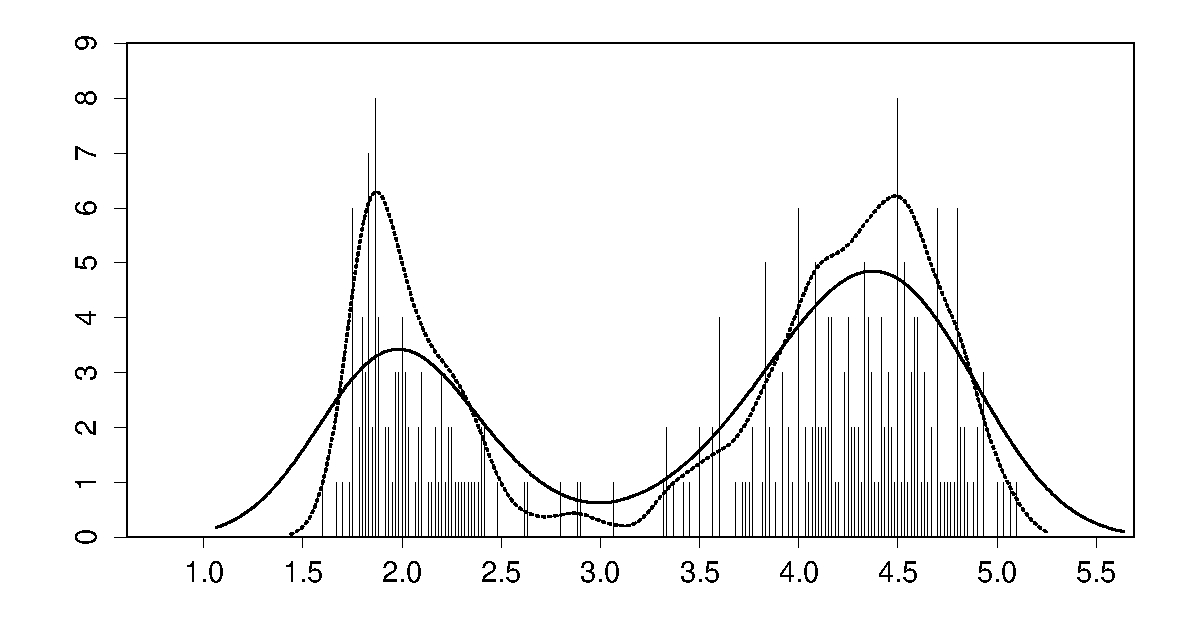
\includegraphics[width=.5\textwidth]{geys-2kern} %<< no file extension
  %%         --- .5\textwidth stands for 50% of text width
  \caption[Geyser data: binned histogram, Silverman's and another
  kernel]%<<-- Legend for the list of figures at the beginning of you thesis
  {Old Faithful Geyser eruption lengths, $n=272$; binned data and two
    (Gaussian) kernel density estimates ($\times 10$) with $h=h^*= .3348$
    and $h= .1$ (dotted).}% legend displayed below the graph.
  \label{fig:geys2}
\end{figure}

\section{To make a proof}
\begin{proof}
  $1 + 1 = 2$
\end{proof}

\section{To include \Rp code}
See information in Appendix~\ref{app:complement}.


\section{Other information}
Put a text between quotes: make sure to use nice quotes, such as ``quote''.

Cite an article or book you refer shortly here, and then listed in the bibliography.
%%--> in file   myReferences.bib  (same directory)
Or mention that \citeauthor{robinson_estimation_1977}  (a person) (two
persons) have already done quite a bit work.

\citeauthor{marvasti_nonuniform_2001}


Referencing a different part of your work: please refer to Appendix \ref{app:complement}.


%%% Local Variables: 
%%% mode: latex
%%% TeX-master: "MasterThesisSfS"
%%% End: 


%%\include{Chapter...}
\chapter{Summary}
\label{s:Summary}

Summarize the presented work. Why is it useful to the research field or institute?


\section{Future Work}
\label{ss:FutureWork}

Possible ways to extend the work.


%%% Local Variables: 
%%% mode: latex
%%% TeX-master: "MasterThesisSfS"
%%% End: 
 

%%%%%%%%%%%%%%%%%%%%%%%%%%%%%%%%%%%%%%%%%%%%%%%%%
%%% Bibliography                              %%%
%%%%%%%%%%%%%%%%%%%%%%%%%%%%%%%%%%%%%%%%%%%%%%%%%
\addtocontents{toc}{\vspace{.5\baselineskip}}
\cleardoublepage
\phantomsection
\addcontentsline{toc}{chapter}{\protect\numberline{}{Bibliography}}
\bibliography{master_thesis_gm}
%% All books from our library (SfS) are already in a BiBTeX file
%% 'Assbib.bib' (included here as well), using
% \bibliography{myReferences,Assbib}
% ---------------------------------- instead of the above



%%%%%%%%%%%%%%%%%%%%%%%%%%%%%%%%%%%%%%%%%%%%%%%%% 
%%% Appendices (if needed, e.g. for R code)   %%%
%%%%%%%%%%%%%%%%%%%%%%%%%%%%%%%%%%%%%%%%%%%%%%%%%
\addtocontents{toc}{\vspace{.5\baselineskip}}
\appendix
\chapter{Complementary information}\label{app:complement}


Additional material. For example long mathematical derivations could be
given in the appendix. Or you could include part of your code that is
needed in printed form. You can add several Appendices to your thesis (as
you can include several chapters in the main part of your work).

\section{Ornstein-Uhlenbeck Process}\label{app:ou}

The autocovariance function of an Ornstein-Uhlenbeck process can be derived by solving the stochastic differential equation (SDE) that defines the process.

Starting with the SDE for an OU process:

$$dX_t = \theta (\mu - X_t)dt + \sigma_w dW_t,$$

where $X_t$ is the value of the process at time $t$, $\theta$ is a positive constant that determines the speed of mean reversion,
$\mu$ is the long-term mean of the process, $\sigma_w$ is the standard deviation of the random shocks, and $W_t$ is a standard Wiener process or Brownian motion.

The solution to the SDE is:

$$ X_t = X_0 e^{-\theta t} + \mu (1-e^{-\theta t}) +
\sigma_w e^{-\theta t} \int_{0}^{t} e^{\theta s} dW_s$$

The process is stationary if $\theta > 0$.
The autocovariance function of an OU process is given by
$Cov(X_t, X_{t-k}) = \frac{\sigma_w^2}{2\theta} e^{-\theta k}$,
where $k\geq 0$ and $\theta > 0$.

This is the same expression as we have obtained in \ref{kernel-matern-ar1}, where
$k(0) = \sigma^2 = \frac{\sigma_w^2}{2\theta}$ and $l=1/\theta$

To see how the Ornstein-Uhlenbeck can be considered a continuous time analogue to the discrete time
AR(1) process one can use the Euler-Maryuama discretization of the process.
Considering again the SDE for an OU process:
$$dX_t = \theta (\mu - X_t)dt + \sigma_w dW_t,$$
The process can be discretized at times $(k \Delta t)_{k \in \mathbb{N}_0}$:

$$ X_{k+1} - X_k = \theta \mu \delta t - \theta X_k \Delta t + \sigma_w (W_{k+1} - W_k)$$

The random variables $(W_{k+1} - W_k)$ are independent and identically distributed normal random variables
with expected value zero and variance $\Delta t$.
Therefore, we can set $\sigma_w (W_{k+1} - W_k) = \sigma_w \sqrt{\Delta t} \epsilon$ with $\epsilon \sim \N(0,1)$
to obtain the following recursion:
$$ X_{k+1} = \theta \mu \Delta t - (\theta \Delta t - 1) X_k + \sigma_w \sqrt{\Delta t} \epsilon$$

The recursion for an AR(1) process is:
$$ X_{k+1} = c + a X_k + b \epsilon$$
Which is identical to the expression above if $c= \theta \mu \Delta t$, $a=1- \theta \Delta t$ and
$b= \sigma_w \sqrt{\Delta t}$



\section{Properties of the Simulated Time Series Samples}\label{sec:properties-of-the-simulated-time-series-samples}

This section presents the distribution of some crucial properties
from the simulated BP time series.
These histograms have been created by drawing 100 samples from the true GP.

The shown property distributions should match those from Section \ref{sec:characteristics-of-the-blood-pressure-time-series}.

\begin{figure}[h!]
    \centering
    \includegraphics[width=0.6\linewidth]{
        Pictures/variance_distribtution/sin_rbf_seasonal_default/09_07_07_12_53/variance_y_true_train_summary.pdf}
    \caption[Distribution of One-Week BP Variance from Simulated Measurements]{
        Distribution of One-Week BP Variance from Simulated Measurements:
    The one-week variance should span from from 16 to 144 mmHg², with an average of 49 mmHg²}
    \label{fig:variance}
\end{figure}

\begin{figure}[h!]
    \centering
    \includegraphics[width=0.6\linewidth]{
       Pictures/variance_distribtution/sin_rbf_seasonal_default/09_07_07_12_53/variance_dip_ampl_summary}
    \caption[Distribution of the Night Dip Magnitude from Simulated Measurements]{
        Distribution of the Night Dip Magnitude from Simulated Measurements:
    Here the night dip magintude is defined as half of the difference between average daytime and nighttime BP measurements.
        Should fall within the range of 0 to 10 mmHg}
    \label{fig:dip_ampl}
\end{figure}



\begin{figure}[h!]
    \centering
    \includegraphics[width=0.6\linewidth]{
       Pictures/variance_distribtution/sin_rbf_seasonal_default/09_07_07_12_53/variance_2.24**2 * Matern(length_scale=3, nu=0.5) * 1**2_summary.pdf}
    \caption[Distribution of the AR Component Variance from Simulated Measurements]{
    Distribution of the AR Component Variance from Simulated Measurements:
    There exists no target values for the variance of the AR component.}
    \label{fig:var_matern}
\end{figure}

\begin{figure}[h!]
    \centering
    \includegraphics[width=0.6\linewidth]{
       Pictures/variance_distribtution/sin_rbf_seasonal_default/09_07_07_12_53/variance_2.24**2 * RBF(length_scale=50) * 1**2_summary.pdf}
    \caption[Distribution of the RBF Component Variance from Simulated Measurements]{
        Distribution of the RBF Component Variance from Simulated Measurements:
        There exists no target values for the variance of teh RBF components}
    \label{fig:var_rbf}
\end{figure}


\begin{figure}[h!]
    \centering
    \includegraphics[width=0.6\linewidth]{
       Pictures/variance_distribtution/sin_rbf_seasonal_default/09_07_07_12_53/variance_14**2 * ExpSineSquared(length_scale=3, periodicity=24) * 1**2_summary.pdf}
    \caption[Distribution of the Periodic Component Variance from Simulated Measurements]{
        Distribution of the Periodic Component Variance from Simulated Measurements:
        The target ranges for the variance of the periodic component are provided in the form of night dip values (see Figure \ref{fig:dip_ampl})}
    \label{fig:var_periodc}
\end{figure}



%
%\section{Including \Rp code with verbatim}
%A simple (rather too simple, see~\ref{App:listings}) way to include code or
%{\it R} output is to use
%\texttt{verbatim}. It just prints the text however it is (including all
%spaces, ``strange'' symbols,...) in a slightly different font.
%\begin{verbatim}
%## loading packages
%library(RBGL)
%library(Rgraphviz)
%library(boot)
%
%## global variables
%X_MAX <- 150
%
%   This allows me to put as many s  p a   c es   as I want.
%I can also use \ and ` and & and all the rest that is usually only
%accepted in the math mode.
%
%I can also make as
%                  many
%             line
%    breaks as
%I want... and
%             where I want.
%\end{verbatim}
%
%But really recommended,  much better is the following:
%
%\section{Including \Rp code with the \emph{listings} package}\label{App:listings}
%However, it is much nicer to use the \emph{listings} package to include \Rp
%code in your report. It allows you to number the lines, color the comments
%differently than the code, and so on.
%All the following is produced by simply writing
%\verb! \lstinputlisting{Pictures/picture.R} !  in your \LaTeX\ ``code'':
%
%\lstinputlisting{Pictures/picture.R}
%
%or \verb!\lstinputlisting{/u/maechler/R/Pkgs/sfsmisc/R/ellipse.R}! :
%
%\lstinputlisting{ellipse.R}% was /u/maechler/R/Pkgs/sfsmisc/R/ellipse.R
%
%\section{Using \texttt{Sweave} (or \texttt{knitr}) to include \Rp code (and more) in your report}
%The easiest (and most elegant) way to include \Rp code and its output (and
%have all your figures up to date with your report) is to use Sweave---or the
%\href{https://cran.R-project.org/package=knitr}{\texttt{knitr}} R package with even more possibilities.
%% You can find an introduction Sweave in \texttt{/u/sfs/StatSoftDoc/Sweave/Sweave-tutorial.pdf}.
%
%Search the web to find lots of intro material on how to use Sweave or
%\href{https://en.wikipedia.org/wiki/Knitr}{knitr (on Wikipedia)}.

%%% Local Variables: 
%%% mode: latex
%%% TeX-master: "MasterThesisSfS"
%%% End: 

\chapter{Yet another appendix....}

\section{Description}
\begin{description}
\item[Something] details.
\item[Something else] other definition.
\end{description}

\section{Tables}
Refer to Table~\ref{tab:example} to see a left justified table with caption
on top.

\begin{table}[ht]
\centering
\caption[Test results]{\label{tab:example}Results.}
\begin{tabular}{ll}
\hline
\textbf{Student} & \textbf{Grade}\\
\hline
Marie  & $6$\\
Alain  & $5.5$\\
Josette  & $4.5$\\
Pierre  & $5$\\
\hline
\end{tabular}
\end{table}

%%% Local Variables: 
%%% mode: latex
%%% TeX-master: "MasterThesisSfS"
%%% End: 

\chapter{2nd Appendix: More sophisticated R code listing} \label{appendix-more-R}

Chapter-wise listing of parts of R code, using
\begin{itemize}
\item \texttt{firstline=n1}
\item \texttt{lastline=n2}
\item \texttt{title=<text>}
\end{itemize}
e.g., for the first example below
\begin{verbatim}
\lstinputlisting[firstline=1,lastline=20,
                 title= \texttt{ellipse.R}]{ellipse.R}
\end{verbatim}
and the second example
\begin{verbatim}
\lstinputlisting[firstline=20,lastline=40,
             title=\texttt{ellipse.R}]{ellipse.R}
\end{verbatim}
% \section{Chapter 2} \label{app 2}

% \lstinputlisting[firstline=1,lastline=77,
% title=\texttt{analytic\_efficiency.R}]{../RCode/analytic_efficiency.R}
% %\lstinputlisting[firstline=,lastline=]{../RCode/???.R}

\bigskip% or even  \clearpage

%-----------------------------------------------------------------------------------------
\section{Chapter 5} \label{app 5}

% \lstinputlisting[firstline=1,lastline=71,
%                  title=\texttt{loss-fn\_rotated.R}]{../RCode/loss-fn_rotated.R}
\lstinputlisting[firstline=1,lastline=20,
                 title= \texttt{ellipse.R}]{ellipse.R}

\medskip
                 
\lstinputlisting[firstline=20,lastline=40,
                 title=\texttt{ellipse.R}]{ellipse.R}
%\lstinputlisting[firstline=,lastline=]{../RCode/???.R}
%\lstinputlisting[firstline=,lastline=]{../RCode/???.R}

% \clearpage
%-----------------------------------------------------------------------------------------
% \section{Chapter 7} \label{app 7}

% \lstinputlisting[firstline=1,lastline=35,
%                  title= \texttt{stat.test} from \texttt{lmrob2-fn.R}]{../RCode/lmrob2-fn.R}
% \lstinputlisting[firstline=41,lastline=194,
%                  title=\texttt{M.optimal.ms} from \texttt{lmrob2-fn.R}]{../RCode/lmrob2-fn.R}
%\lstinputlisting[firstline=,lastline=]{../RCode/???.R}
%-----------------------------------------------------------------------------------------

%%% Local Variables:
%%% mode: latex
%%% TeX-master: "MasterThesisSfS"
%%% End:



%% Epilogue (optional)
\addtocontents{toc}{\vspace{.5\baselineskip}}
\cleardoublepage
\phantomsection
\addcontentsline{toc}{chapter}{\protect\numberline{}{Epilogue}}
\markboth{Epilogue}{Epilogue}
\chapter*{Epilogue}
\label{s:Epilogue}

A few final words.



%%% Local Variables: 
%%% mode: latex
%%% TeX-master: "MasterThesisSfS"
%%% End: 



%%%%%%%%%%%%%%%%%%%%%%%%%%%%%%%%%%%%%%%%%%%%%%%%%% 
%%% Declaration of originality (Do not remove!)%%%
%%%%%%%%%%%%%%%%%%%%%%%%%%%%%%%%%%%%%%%%%%%%%%%%%%
%% Instructions:
%% -------------
%% fill in the empty document confirmation-originality.pdf electronically
%% print it out and sign it
%% scan it in again and save the scan in this directory with name
%% confirmation-originality-scan.pdf 
%%
%% General info on plagiarism:
%% https://www.ethz.ch/students/en/studies/performance-assessments/plagiarism.html 
\cleardoublepage
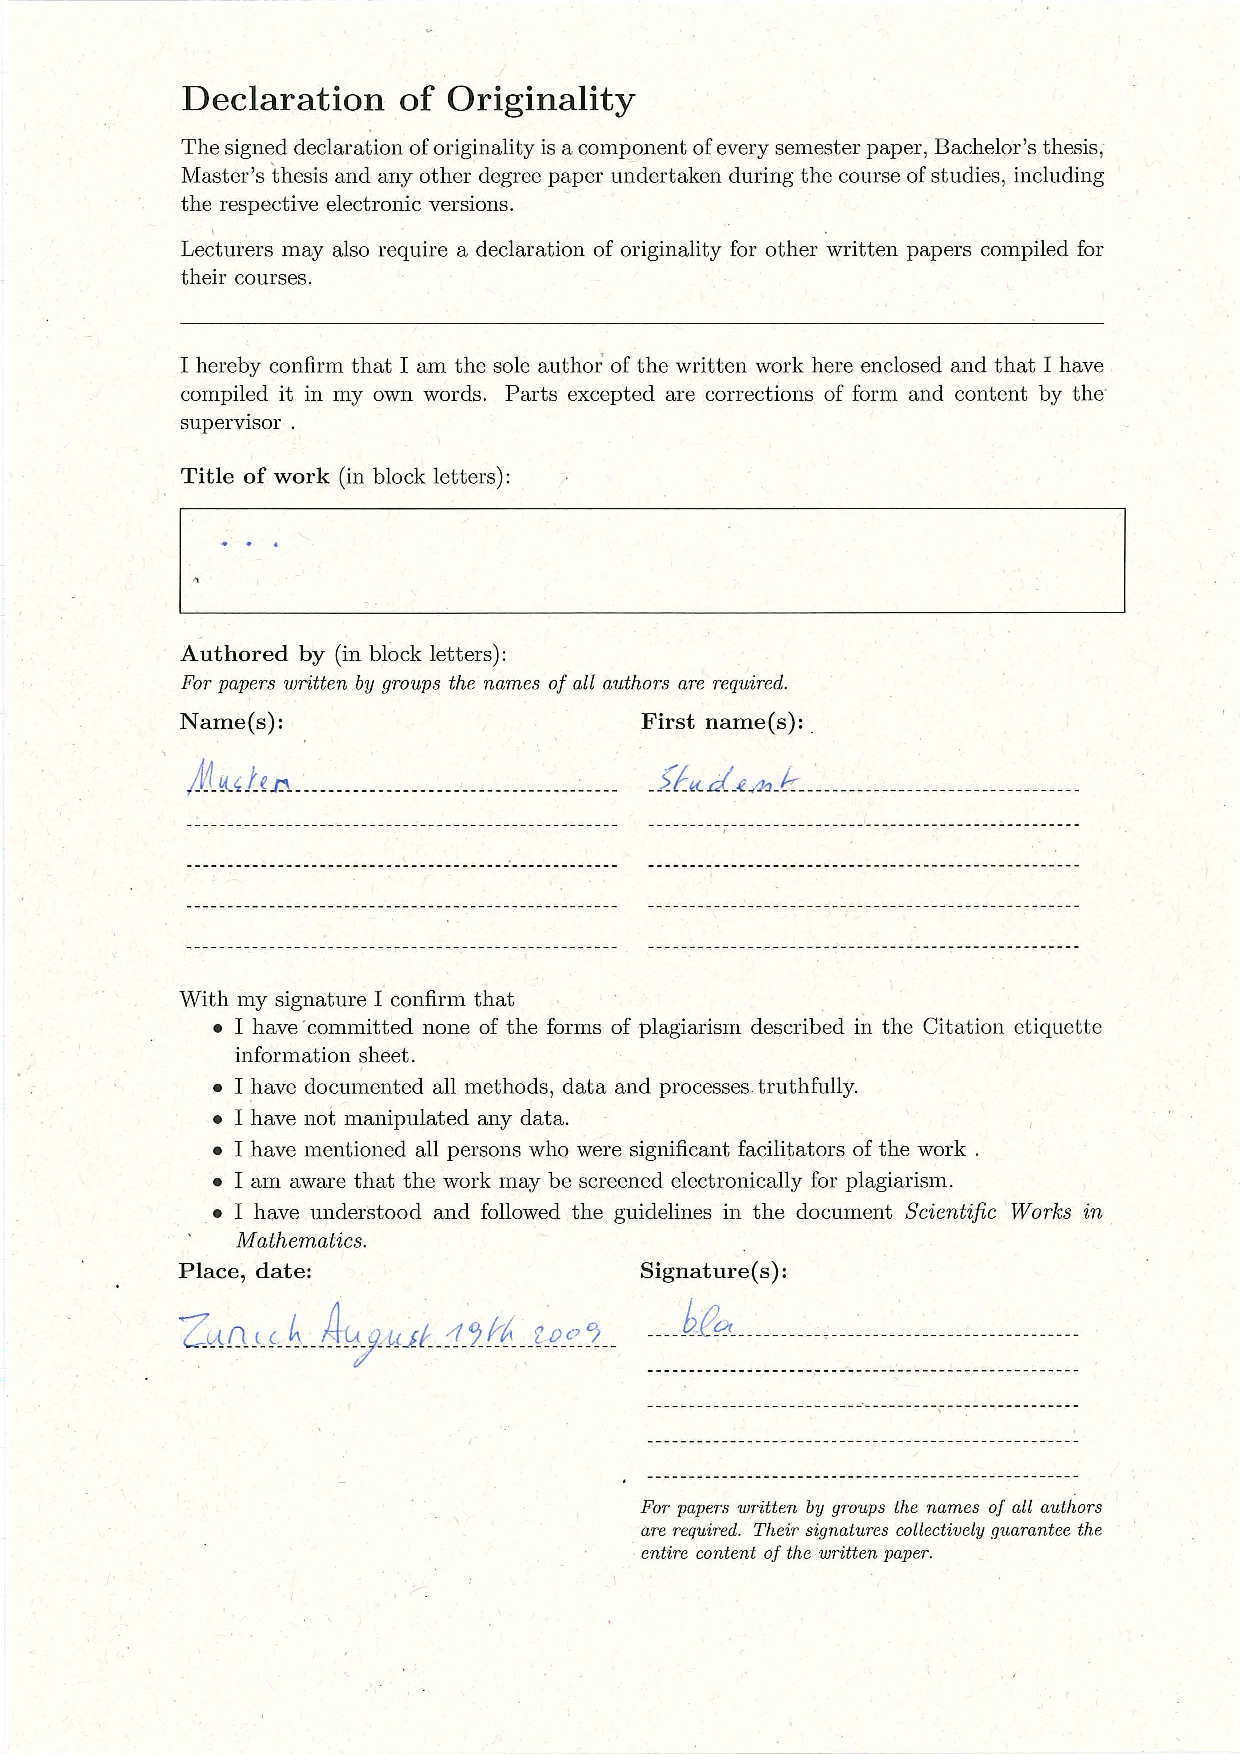
\includepdf[pages={-}, frame=true,scale=1]{confirmation-originality-scan.pdf}
\end{document}

%%% Local Variables:
%%% mode: latex
%%% TeX-master: "MasterThesisSfS"
%%% End:
